% Disclosure method on the film request (an illustration of Algorithm 1; the two results are the real sakila_1 values of the teaser).
% Shared setup for the diagrams (teaser, pipeline, worked). Built with XeLaTeX so that all text is Arial, in black.
% Sizes match the paper's acmart sigconf sizes (\footnotesize 7 pt); the smallest text is 6 pt.
\documentclass[border=0.5pt]{standalone}
\usepackage{fontspec}
\setmainfont{Arial}\setsansfont{Arial}\setmonofont{Menlo}[Scale=MatchLowercase]
\usepackage{unicode-math}\setmathfont{FiraMath-Regular.otf}
\usepackage{booktabs}
\usepackage{tikz}
\usetikzlibrary{arrows.meta,calc,positioning,fit,backgrounds,shapes.geometric}
\renewcommand\large{\fontsize{10}{12}\selectfont}
\renewcommand\small{\fontsize{8}{10}\selectfont}
\renewcommand\footnotesize{\fontsize{7}{8.4}\selectfont}
\renewcommand\scriptsize{\fontsize{6.5}{7.6}\selectfont}
\renewcommand\tiny{\fontsize{6}{7}\selectfont}
\newcommand{\nohyph}{\hyphenpenalty=10000\exhyphenpenalty=10000\relax}
\newcommand{\sql}[1]{\texttt{#1}}
% the edited SQL clause, highlighted as in AMBROSIA and the test-suite paper; plain check and cross marks
\newcommand{\hl}[2]{{\setlength{\fboxsep}{0.7pt}\colorbox{#1f}{\vphantom{Ay}\texttt{#2}}}}
\newfontfamily\markfont{Arial Unicode MS}\newcommand{\yes}{{\markfont ✓}}\newcommand{\no}{{\markfont ✗}}
% math letters in Arial italic; the open-request circle is drawn; only the arrow comes from Fira Math
\newcommand{\vq}[1]{\textit{q}\textsubscript{#1}}\newcommand{\vp}[1]{\textit{p}\textsubscript{#1}}\newcommand{\vo}{\mbox{\textit{q}\hspace{0.3pt}\raisebox{-0.25ex}{\tikz[baseline=0pt]\draw[line width=0.45pt] (0,1.1pt) circle (1.1pt);}}}
% box lines: A (blue) and B (orange) as in the data figures; neutral lines grey. Text is always black.
% colors as in AMBROSIA's and AmbiQT's diagrams (draw.io palette): interpretation A blue, interpretation B orange, code blocks light gray
\definecolor{sbA}{HTML}{6C8EBF}\definecolor{sbB}{HTML}{D79B00}\definecolor{sbAf}{HTML}{DAE8FC}\definecolor{sbBf}{HTML}{FFE6CC}\definecolor{sbline}{HTML}{4D4D4D}
\definecolor{sbfill}{HTML}{F5F5F5}

\begin{document}
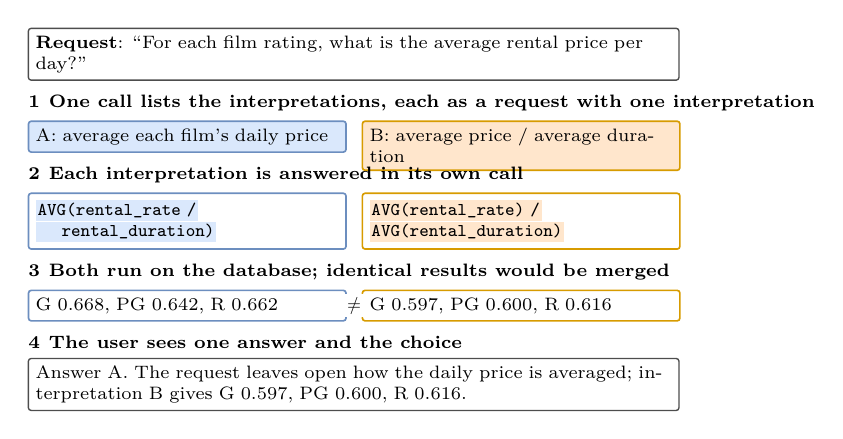
\begin{tikzpicture}[x=1cm, y=1cm, font=\scriptsize, >=Stealth, line width=0.5pt,
  st/.style={font=\scriptsize\bfseries, anchor=north west, inner sep=0pt},
  rd/.style={draw=#1, line width=0.6pt, rounded corners=1pt, inner sep=2.6pt, align=left, text width=3.85cm, anchor=north west},
  bx/.style={draw=sbline, rounded corners=1pt, inner sep=2.6pt, align=left, text width=8.08cm, anchor=north west},
  arr/.style={->, draw=sbline}]
\node[bx] (q) at (0,0) {\textbf{Request}: ``For each film rating, what is the average rental price per day?''};
\node[st] (s1) at ([yshift=-5pt]q.south west) {1\enspace One call lists the interpretations, each as a request with one interpretation};
\node[rd=sbA, fill=sbAf] (a) at ([yshift=-3pt]s1.south west) {A: average each film's daily price};
\node[rd=sbB, fill=sbBf] (b) at ([xshift=4.24cm]a.north west) {B: average price / average duration};
\node[st] (s2) at ([yshift=-5pt]a.south west) {2\enspace Each interpretation is answered in its own call};
\node[rd=sbA] (pa) at ([yshift=-3pt]s2.south west) {\hl{sbA}{AVG(rental\_rate /}\\\hl{sbA}{\ \ \ \ rental\_duration)}};
\node[rd=sbB] (pb) at ([xshift=4.24cm]pa.north west) {\hl{sbB}{AVG(rental\_rate) /}\\\hl{sbB}{AVG(rental\_duration)}};
\node[st] (s3) at ([yshift=-5pt]pa.south west) {3\enspace Both run on the database; identical results would be merged};
\node[rd=sbA] (ra) at ([yshift=-3pt]s3.south west) {G 0.668, PG 0.642, R 0.662};
\node[rd=sbB] (rb) at ([xshift=4.24cm]ra.north west) {G 0.597, PG 0.600, R 0.616};
\node[font=\scriptsize, fill=white, inner sep=1pt] at ($(ra.east)!0.5!(rb.west)$) {$\neq$};
\node[st] (s4) at ([yshift=-5pt]ra.south west) {4\enspace The user sees one answer and the choice};
\node[bx] (o) at ([yshift=-3pt]s4.south west) {Answer A. The request leaves open how the daily price is averaged; interpretation B gives G 0.597, PG 0.600, R 0.616.};
\end{tikzpicture}
\end{document}
